\documentclass[12pt,]{article}
\usepackage{lmodern}
\usepackage{amssymb,amsmath}
\usepackage{ifxetex,ifluatex}
\usepackage{fixltx2e} % provides \textsubscript
\ifnum 0\ifxetex 1\fi\ifluatex 1\fi=0 % if pdftex
  \usepackage[T1]{fontenc}
  \usepackage[utf8]{inputenc}
\else % if luatex or xelatex
  \ifxetex
    \usepackage{mathspec}
  \else
    \usepackage{fontspec}
  \fi
  \defaultfontfeatures{Ligatures=TeX,Scale=MatchLowercase}
\fi
% use upquote if available, for straight quotes in verbatim environments
\IfFileExists{upquote.sty}{\usepackage{upquote}}{}
% use microtype if available
\IfFileExists{microtype.sty}{%
\usepackage{microtype}
\UseMicrotypeSet[protrusion]{basicmath} % disable protrusion for tt fonts
}{}
\usepackage[margin=1in]{geometry}
\usepackage{hyperref}
\hypersetup{unicode=true,
            pdfauthor={Xuan Son Le (4669361), Freie Universität Berlin},
            pdfborder={0 0 0},
            breaklinks=true}
\urlstyle{same}  % don't use monospace font for urls
\usepackage{color}
\usepackage{fancyvrb}
\newcommand{\VerbBar}{|}
\newcommand{\VERB}{\Verb[commandchars=\\\{\}]}
\DefineVerbatimEnvironment{Highlighting}{Verbatim}{commandchars=\\\{\}}
% Add ',fontsize=\small' for more characters per line
\usepackage{framed}
\definecolor{shadecolor}{RGB}{248,248,248}
\newenvironment{Shaded}{\begin{snugshade}}{\end{snugshade}}
\newcommand{\KeywordTok}[1]{\textcolor[rgb]{0.13,0.29,0.53}{\textbf{#1}}}
\newcommand{\DataTypeTok}[1]{\textcolor[rgb]{0.13,0.29,0.53}{#1}}
\newcommand{\DecValTok}[1]{\textcolor[rgb]{0.00,0.00,0.81}{#1}}
\newcommand{\BaseNTok}[1]{\textcolor[rgb]{0.00,0.00,0.81}{#1}}
\newcommand{\FloatTok}[1]{\textcolor[rgb]{0.00,0.00,0.81}{#1}}
\newcommand{\ConstantTok}[1]{\textcolor[rgb]{0.00,0.00,0.00}{#1}}
\newcommand{\CharTok}[1]{\textcolor[rgb]{0.31,0.60,0.02}{#1}}
\newcommand{\SpecialCharTok}[1]{\textcolor[rgb]{0.00,0.00,0.00}{#1}}
\newcommand{\StringTok}[1]{\textcolor[rgb]{0.31,0.60,0.02}{#1}}
\newcommand{\VerbatimStringTok}[1]{\textcolor[rgb]{0.31,0.60,0.02}{#1}}
\newcommand{\SpecialStringTok}[1]{\textcolor[rgb]{0.31,0.60,0.02}{#1}}
\newcommand{\ImportTok}[1]{#1}
\newcommand{\CommentTok}[1]{\textcolor[rgb]{0.56,0.35,0.01}{\textit{#1}}}
\newcommand{\DocumentationTok}[1]{\textcolor[rgb]{0.56,0.35,0.01}{\textbf{\textit{#1}}}}
\newcommand{\AnnotationTok}[1]{\textcolor[rgb]{0.56,0.35,0.01}{\textbf{\textit{#1}}}}
\newcommand{\CommentVarTok}[1]{\textcolor[rgb]{0.56,0.35,0.01}{\textbf{\textit{#1}}}}
\newcommand{\OtherTok}[1]{\textcolor[rgb]{0.56,0.35,0.01}{#1}}
\newcommand{\FunctionTok}[1]{\textcolor[rgb]{0.00,0.00,0.00}{#1}}
\newcommand{\VariableTok}[1]{\textcolor[rgb]{0.00,0.00,0.00}{#1}}
\newcommand{\ControlFlowTok}[1]{\textcolor[rgb]{0.13,0.29,0.53}{\textbf{#1}}}
\newcommand{\OperatorTok}[1]{\textcolor[rgb]{0.81,0.36,0.00}{\textbf{#1}}}
\newcommand{\BuiltInTok}[1]{#1}
\newcommand{\ExtensionTok}[1]{#1}
\newcommand{\PreprocessorTok}[1]{\textcolor[rgb]{0.56,0.35,0.01}{\textit{#1}}}
\newcommand{\AttributeTok}[1]{\textcolor[rgb]{0.77,0.63,0.00}{#1}}
\newcommand{\RegionMarkerTok}[1]{#1}
\newcommand{\InformationTok}[1]{\textcolor[rgb]{0.56,0.35,0.01}{\textbf{\textit{#1}}}}
\newcommand{\WarningTok}[1]{\textcolor[rgb]{0.56,0.35,0.01}{\textbf{\textit{#1}}}}
\newcommand{\AlertTok}[1]{\textcolor[rgb]{0.94,0.16,0.16}{#1}}
\newcommand{\ErrorTok}[1]{\textcolor[rgb]{0.64,0.00,0.00}{\textbf{#1}}}
\newcommand{\NormalTok}[1]{#1}
\usepackage{graphicx,grffile}
\makeatletter
\def\maxwidth{\ifdim\Gin@nat@width>\linewidth\linewidth\else\Gin@nat@width\fi}
\def\maxheight{\ifdim\Gin@nat@height>\textheight\textheight\else\Gin@nat@height\fi}
\makeatother
% Scale images if necessary, so that they will not overflow the page
% margins by default, and it is still possible to overwrite the defaults
% using explicit options in \includegraphics[width, height, ...]{}
\setkeys{Gin}{width=\maxwidth,height=\maxheight,keepaspectratio}
\IfFileExists{parskip.sty}{%
\usepackage{parskip}
}{% else
\setlength{\parindent}{0pt}
\setlength{\parskip}{6pt plus 2pt minus 1pt}
}
\setlength{\emergencystretch}{3em}  % prevent overfull lines
\providecommand{\tightlist}{%
  \setlength{\itemsep}{0pt}\setlength{\parskip}{0pt}}
\setcounter{secnumdepth}{5}
% Redefines (sub)paragraphs to behave more like sections
\ifx\paragraph\undefined\else
\let\oldparagraph\paragraph
\renewcommand{\paragraph}[1]{\oldparagraph{#1}\mbox{}}
\fi
\ifx\subparagraph\undefined\else
\let\oldsubparagraph\subparagraph
\renewcommand{\subparagraph}[1]{\oldsubparagraph{#1}\mbox{}}
\fi

%%% Use protect on footnotes to avoid problems with footnotes in titles
\let\rmarkdownfootnote\footnote%
\def\footnote{\protect\rmarkdownfootnote}

%%% Change title format to be more compact
\usepackage{titling}

% Create subtitle command for use in maketitle
\newcommand{\subtitle}[1]{
  \posttitle{
    \begin{center}\large#1\end{center}
    }
}

\setlength{\droptitle}{-2em}
  \title{\textbf{Logistische Regression}}
  \pretitle{\vspace{\droptitle}\centering\huge}
  \posttitle{\par}
  \author{Xuan Son Le (4669361), Freie Universität Berlin}
  \preauthor{\centering\large\emph}
  \postauthor{\par}
  \predate{\centering\large\emph}
  \postdate{\par}
  \date{02/04/2018}


\begin{document}
\maketitle

\begin{center}\rule{0.5\linewidth}{\linethickness}\end{center}

\textbf{Abstract}: Im Rahmen der Abschlussarbeit des Moduls
Programmieren mit R im Wintersemester 2017/2018 an der Freie Universität
Berlin wird für diese Arbeit die statistische Methode namens binäres
Logit-Modell ausgewählt. Diese Arbeit besteht aus zwei großen
Hauptteilen: der Theorieteil, wobei die ausgewählte Methode theoretisch
vorgestellt wird und der Implementierungsteil, welcher die Erklärung der
Funktionalität vom selbst entwickelten Paket beinhaltet. Im Theorieteil
wird zunächst ein Überblick über die grundliegende Funktionsweise vom
(binären) Logit-Modell widergegeben. Die Grundidee von Generalisierten
linearen Modellen wird anschließend kurz eingeführt, bevor der Aufbau
vom binären Logit-Modell durch das Maximum Likelihood Verfahren
vorgenommen wird. Demzufolge folgt die Interpretation der Koeffizienten
vom binären Logit-Modell. Schließlich werden im Implementierungsteil
alle Funktionen vom R-Paket schritterweise vorgestellt.

\textbf{Keywords:} \emph{Logit-Modell, logistische Regression, Paket, R}

\begin{center}\rule{0.5\linewidth}{\linethickness}\end{center}

\newpage

\section{Motivation}\label{motivation}

Die Anwendung von der klassischen linearen Regression ist für binäre
(binomiale oder dichotome) Zielvariable (Response- oder zu erklärende
Variable), welche lediglich zwei Werte (ja/nein, mänlich/weiblich,
erfolgreich/nicht erfolgreich, etc.) annehmen kann, nicht mehr geeignet,
da die Zielvariable von der linearen Regression metrisch skaliert ist.
Oft wird binäre Variable als 0/1-Variable kodiert, das heißt sie nimmt
nur den Wert 0 oder 1 an. Die folgende Grafik stellt den Ansatz
graphisch dar, binäre Variable durch lineare Regression zu modellieren:

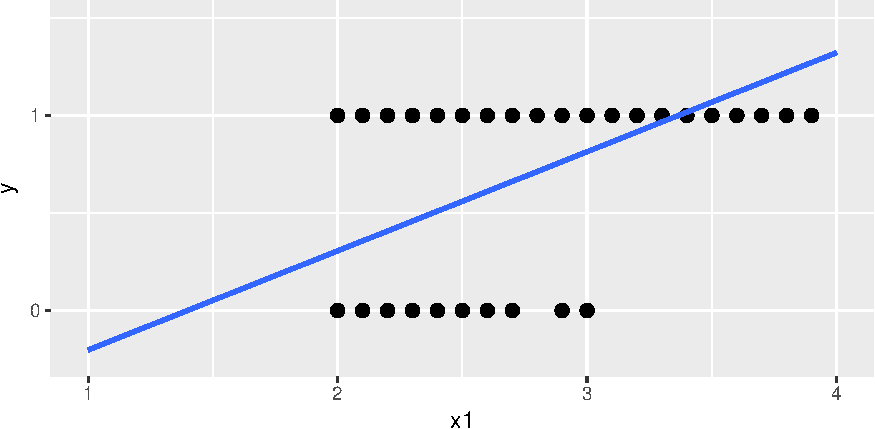
\includegraphics{logisticRegression_files/figure-latex/unnamed-chunk-1-1.pdf}

Graphisch lässt sich festlegen, dass die lineare Regression den
Wertebereich {[}0,1{]} von binären Responsevariablen sehr schnell
verlässt. Wenn die Annahmen von der linearen Regression noch in Betracht
gezogen werden, ergeben sich darüber hinaus noch folgende Probleme (vgl.
\ldots{}): \emph{ } *

Aus diesen Gründen wird ein ganz anderer Ansatz benötigt, um binäre
Zielvariable zu modellieren, nämlich das binäre Logit-Modell, welches
ebenfalls als binäre logistische Regression oder binäres logistisches
Regressionsmodell bezeichnet werden kann. In der Statistik lassen sich
Logit-Modelle noch in multinomiale und kumulative Logit-Modelle
aufteilen, je nachdem ob die abhängige Variable multinominal- oder
ordinalskaliert sind . Diese Arbeit beschäftigt sich mit dem binären
Logit-Modell, welches den Zusammenhang zwischen einer binären abhängigen
Variable und einer/mehreren unabhängigen Variablen untersucht. Bei allen
Arten von Logit-Modellen können die unabhängigen Variablen (erklärende
oder Kovariablen) beliebig skaliert sein.

Im Unterschied zu der klassischen linearen Regression, welche den wahren
Wert einer Zielvariable vorhersagt, interessiert sich das binäre
Logit-Modell eher für die Wahrscheinlichkeit, dass die Zielvariable den
Wert 1 annimmt. Das Hauptziel vom binären Logit-Modell ist es, die
Wahrscheinlichkeit für den Eintritt der Zielvariable vorherzusagen.
Dadurch soll die folgende theoretische Fragestellung beantwortet werden:
\emph{Wie stark ist der Einfluss von den unabhängigen (erklärenden)
Variablen auf die Wahrscheinlichkeit, dass die abhängige (zu erklärende
/ Response) Variable eintritt beziehungsweise den Wert 1 annimmt?} In
der Praxis kann diese Fragestellung beispielsweise so formuliert werden:
``Haben Alter, Geschlecht, Berufe oder andere Merkmale der Kunden
Einfluss auf die Wahrscheinlichkeit, dass sie ein Kredit rechtzeitig
zurückzahlen?'' oder ``Lässt sich die Wahrscheinlichkeit, dass es
regnet, durch die Temparatur, die Windstärke oder
Sonnenstrahlungsintensität vorhersagen?''.

\section{Das binäre Logit-Modell}\label{das-binare-logit-modell}

\subsection{Modellspezifikation}\label{modellspezifikation}

Das Logit-Modell ist eine Methode aus der Algorithmenklasse namens
\emph{Generalisierte Lineare Modelle} (engl. generalized linear model,
kurz GLM), welche eine Verallgemeinerung des klassischen linearen
Regressionsmodells anstrebt. Dazu gehören noch die klassische lineare
Regression, Probitmodell und Poisson-Regression. Die Grundidee von GLM
ist die Transformation der linearen Regressionsgleichung, so dass der
Wertebereich der vorhergesagten Zielvariable dem gewünschten entspricht.
Die Theorie von GLMs wurde von Nelder und Wedderburn entwickelt.

Gegeben seien n unabhängige Beobachtungen \(y_1, y_2, ...,y_n\) der
binären Zielvariable \(\mathbf{Y}\). Ein Verteilungsmodell für
\(\mathbf{Y}\) ist die Binomialverteilung:
\(\mathbf{Y}_i \sim B(1, \pi_i)\) mit \(\pi_i = P(Y_i = 1)\).Für diese
Arbeit wird \(\pi_i = (\pi_1, \pi_2, ..., \pi_n)\) als die
Eintrittwahrscheinlichkeit von der einzelnen \(\mathbf{Y}_i\) benannt.
Weiterhin seien p erklärende Variablen
\(\mathbf{X}_0,\mathbf{X}_1,..,\mathbf{X}_k\) gegeben mit jeweils n
unabhängigen Beobachtungen
\(\mathbf{X}_j = (x_{1j}, x_{2j},..., x_{nj})\) mit j \(\in\)
\{1,2,..,k\} gegeben. Daraus ergeben sich p Koeffizienten
\(\beta = (\beta_0, \beta_1, \beta_2,..., \beta_p)\), welche die Stärke
den Zusammenhang zwischen die einzelne erklärende Variable mit der
Zielvariable widerspiegeln. Dabei ist es sinnvoll, diese in einer
Designmatrix \(\mathbf{X}\) zu speichern. Da der Interzept (\(\beta_0\))
ebenfalls geschätzt werden soll, sind alle Werte der ersten Spalte von X
gleich Eins, also \(x_{10} = x_{20} = ... = x_{n0} = 1\).
Zusammengefasst lässt sich die Designmatrix wie folgt darstellen: \[
\mathbf{X} =
 \begin{pmatrix}
    1 & x_{11} & x_{12} & \cdots & x_{1k} \\
    1 & x_{21} & x_{22} & \cdots & x_{2k} \\
    1 & x_{31} & x_{32} & \cdots & x_{3k} \\
    \vdots  & \vdots  & \vdots & \ddots & \vdots \\
    1 & x_{n1} & x_{n2} & \cdots & x_{nk}
 \end{pmatrix}
\] Die dazugehörige lineare Regressionsgleichung lautet:
\(\mathbf{Y} = \mathbf{X}.\beta + \epsilon\) mit
\(\epsilon = (\epsilon_1, \epsilon_2, \epsilon_3, ..., \epsilon_n)\) als
die Abweichung der einzelnen Schätzungen gegenüber dem wahren Wert. Die
einzelne Beobachtung lässt sich wie folgt darstellen:
\[y_i = \beta_0 + \beta_1.x_{i2} + \beta_2.x_{i3} + ... + \beta_k.x_{ik} + \epsilon_i \qquad \forall_i = 1,2,3,...,n\]

Um die Werte im Bereich der reellen Zahlen von der linearen Regression
auf dem Wertebereich von Wahrscheinlichkeiten zwischen 0 und 1 zu
beschränken, sollte die rechte Seite der Gleichung transformiert werden.
Das Ziel ist es, eine sinnvolle Verteilungsfunktion (Responsefunktion)
zu finden, deren Wertebereich in {[}0,1{]} liegt:
\(\pi_i = P(\mathbf{Y_i} = 1) = F(\beta_0 + \beta_1.x_{i2} + \beta_2.x_{i3} + ... + \beta_k.x_{ik}) = F(\eta_i)\).
Der lineare Prädikator
\(\eta_i = \beta_0 + \beta_1.x_{i2} + \beta_2.x_{i3} + ... + \beta_k.x_{ik}\)
wird ebenfalls als Linkfunktion genannt, weil dadurch eine Verbindung
(Link) zwischen der Eintrittwahrscheinlichkeit und den unabhängigen
Variablen erfolgt wird. Für das binäre Logit-Modell wird anstelle der
Responsefunktion die standardisierte logistische Verteilung verwendet:
\[
F(\eta_i) = Logist(\eta_i) = \frac{\exp(\eta_i)}{1 + \exp(\eta_i)} 
\] Da durch die Responsefunktion die Eintrittwahrscheinlichkeit
\(\pi_i\) modelliert werden soll, ergibt sich die Gleichung für das
binäre Logit-Modell wie folgt: \[
\pi_i = \frac{\exp(\eta_i)}{1 + \exp(\eta_i)} = \frac{\exp(\beta_0 + \beta_1.x_{i2} + \beta_2.x_{i3} + ... + \beta_k.x_{ik})}{1 + \exp(\beta_0 + \beta_1.x_{i2} + \beta_2.x_{i3} + ... + \beta_k.x_{ik})}
\] Dabei kann \(\pi_i\) maximal den Wert 1 nehmen, wenn \(\exp(\eta_i)\)
sehr groß ist und minimal den Wert 0, wenn \(\exp(\eta_i)\) sehr nah
rechts von 0 liegt. \(\exp(\eta_i)\) kann nicht negativ sein. Diese
Gleichung erfüllt somit die Anforderung bezüglich dem Wertebereich von
Wahrscheinlichkeiten.

Soll die Gleichung nach dem linearen Prädikator \(\eta_i\) gelöst
werden, ergibt sich schließlich die Logit-Linkfunktion: \[
\begin{aligned}
\pi_i.(1 + \exp(\eta_i)) &= \exp(\eta_i) \\
\Leftrightarrow \pi_i + \pi_i.\exp(\eta_i) &= \exp(\eta_i) \\
\Leftrightarrow \pi_i &= \exp(\eta_i) - \pi_i.\exp(\eta_i)  \\
\Leftrightarrow \pi_i &= \exp(\eta_i).(1-\pi_i) \\
\Leftrightarrow \exp(\eta_i) &= \frac{\pi_i}{1-\pi_i} \\
\Leftrightarrow \eta_i &= \ln(\frac{\pi_i}{1-\pi_i}) \\
\end{aligned}
\]

Es gilt nämlich: \[
\beta_0 + \beta_1.x_{i2} + \beta_2.x_{i3} + ... + \beta_k.x_{ik} = \ln(\frac{\pi_i}{1-\pi_i})
\]

\subsection{Maximum Likelihood
Schätzung}\label{maximum-likelihood-schatzung}

Ähnlich wie bei der linearen Regression muss bei dem binären
Logit-Modell die unbekannten Parameter \(\beta_i\) (i =
0,1,2,\ldots{},k) ebenfalls geschätzt werden. Bei der klassischen
linearen Regression wird die Methode der Kleinsten Quadrate (engl.
\emph{method of least squares}, kurz KQ-Methode) genutzt, um eine
Regressionslinie zu bestimmen, welche die Summe der quadratischen
Abweichungen von den beobachteten Punkten minimiert. Da bei dem binären
Logit-Modell nicht der wahre Wert der Zielvariable sondern die
Eintrittswahrscheinlichkeit geschätzt wird, ist die Abweichung zwischen
dem wahren Wert und dem geschätzten Wert nicht mehr aussagekräftig wie
bei der linearen Regression. Die Koeffizienten müssen anders geschätzt
werden. Dementsprechend wird bei dem binären Logit-Modell die sogenannte
Maximum Likelihood Schätzung (kurz ML-Schätzung) eingesetzt. Abbildung
.. zeigt ein Beispiel mit zwei mögliche binäre logistiche
Regressionskurven, die durch die Maximum Likelihood optimiert werden
sollen.

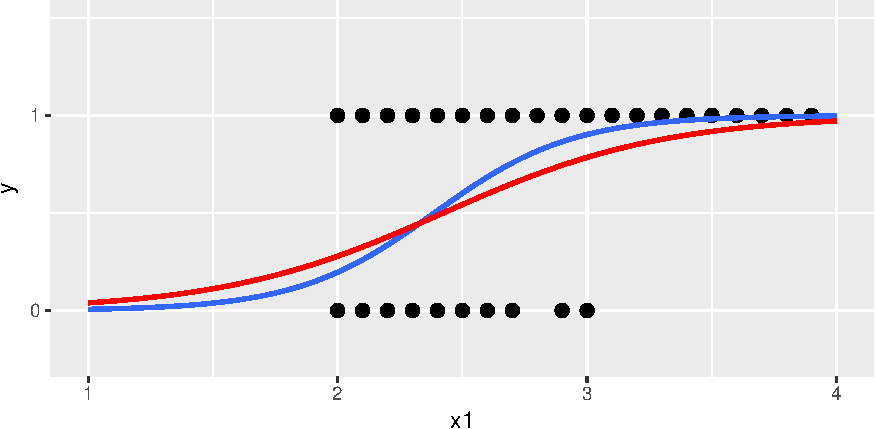
\includegraphics{logisticRegression_files/figure-latex/unnamed-chunk-2-1.pdf}

Das Ziel der ML-Schätzung besteht darin, die (Log-)Likelihood-Funktion
zu maximieren. Im Folgenden wird die Vorgehensweise zum Aufbau der
Log-Likelihood-Funktion wiedergegeben.

Gegeben sei \(y_i = 1\) mit der Eintrittswahrscheinlichkeit \(\pi_i\),
und \(y_i = 0\) mit der Gegenwahrscheinlichkeit \((1-\pi_i)\). Die
Likelihood-Funktion lässt sich wie folgt definieren: \[
\mathcal{L}(\beta) = {\prod_{i=1}^{n} \pi_i^{y_i}.(1-\pi_i)^{1-y_i}}
\] Wenn \(y_i\) gleich 1 ist, ergibt sich für die betroffene Beobachtung
die Eintrittswahrscheinlichkeit \(\pi_i\) und umgekehrt. Das Likelihood
ist gleich die Multiplikation der Wahrscheinlichkeiten von allen
Beobachtungen. Dieses soll maximiert werden.

Da \(\pi_i\) von dem linearen Prädikator \(\eta_i\) anhängt, ist die
Likelihood-Funktion von \(\beta\) abhängig. Wird
\(\pi_i = \frac{\exp(\eta_i)}{1 + \exp(\eta_i)}\) in die
Likelihood-Funktion eingesetzt, ergibt sich:

\[
\mathcal{L}(\beta) = {\prod_{i=1}^{n} \Bigg[ \Big( \frac{\exp(\eta_i)}{1 + \exp(\eta_i)} \Big)^{y_i}.\Big(1-\frac{\exp(\eta_i)}{1 + \exp(\eta_i)}\Big)^{1-y_i}}\Bigg]
\]

Der Versuch, diese Gleichung zu differenzieren und nach \(\beta\) zu
lösen, um die Nullpunkt zu lösen, ist extrem aufwendig. Wegen den
exponentialen Komponenten kann die logistische Funktion aus der
Mathematik zur Vereinfachung der Likelihood-Funktion Einsatz finden. Da
die logistische Funktion eine monotone Funktion ist, entspricht jedes
Maximum von der Likelihood-Funktion dem Maximum von der
Log-Likelihood-Funktion und umgekehrt. Es gelgen für den Logarithmus
folgende Regelungen: \[
\begin{aligned}
(1) \quad &\ln(\prod_{i=1}^{n}x_i) = \ln(x_1.x_2...x_n.) = \ln(x_1) + \ln(x_2) + ... + \ln(x_n) = \sum_{i=1}^{n} \ln(x_i) \\
(2) \quad &\ln(x^\alpha) = \alpha.\ln(x) \\
(3) \quad &\ln(\frac{x}{y}) = \ln(x) - \ln(y) \\
\end{aligned}
\]

Dementsprechend lässt die Likelihood-Funktion wie folgt
logarithmisieren: \$\$

\$\$

\subsection{Intepretation der
Koeffizienten}\label{intepretation-der-koeffizienten}

Die Bruchrechnung \(\frac{\pi_i}{1-\pi_i}\) spielt bei dem binären
Logit-Modell eine besondere Rolle, weil sie mit der
Eintrittswahrscheinlichkeit sehr

\section{Implementierung in R}\label{implementierung-in-r}

Im Folgenden wird die Funktionalität von dem Paket \textbf{logitModell}
erklärt, welches zum Ziel setzt, die Grundidee hinter dem binären
Logit-Modell programmiert darzustellen. Das Paket besteht aus dem
R-Code, welcher anhand dem manuell berechneten Maximum Likelihood ein
Objekt von der Klasse \emph{logitMod} erstellt und anschließend drei S3
Methoden für diese Klasse (print, summary und plot) definiert, und einer
Vignette, welche den R-Code anhand einem konkreten Beispiel ausführt.
Dieser Beispieldatensatz wird im Folgenden verwendet, um die Richtigkeit
und Vollständigkeit der Ergebnisse der implementierten Methode im
Vergleich zu der R-Standardmethode für Logit-Modell \emph{glm(\ldots{},
family = ``binomial'')} zu testen. Die binäre Responsevariable heißt
\emph{admit}, welche besagt ob ein Kandidat eine Zulassung bekommt.
Zudem enthält der Datensatz drei unabhängige Variablen: \emph{gre},
\emph{gpa} (metrisch) und \emph{rank} (kategorial). Der Datensatz soll
ein Modell unterstützen, welche die Abhängigkeit von der
Wahrscheinlichkeit einer Zulassung von der Abschlussnote, GRE-Note sowie
dem Ruf von der angestrebten Institution.

\subsection{Beispieldatensatz}\label{beispieldatensatz}

Zunächst wird der Datensatz importiert. Dabei wird die Zielvariable aus
dem Datensatz entnommen und in einem Vektor gespeichert. Da diese schon
als 0/1-Variable vorgegeben wird, besteht es in diesem Fall keine
Notwendigkeit, die Zielvariable zu faktorisieren. Der Code funktioniert
allerdings ebenfalls mit Zielvariable, welche zum Beispiel als
weiblich/männlich oder Erfolg/kein Erfolg kodiert wird und transformiert
diese in eine 0/1-Variable.

\begin{Shaded}
\begin{Highlighting}[]
\CommentTok{# sei y die eingegebene Zielvariable}
\ControlFlowTok{if}\NormalTok{ (}\OperatorTok{!}\NormalTok{(}\DecValTok{0} \OperatorTok\StringTok{ }\NormalTok{y }\OperatorTok{&&}\StringTok{ }\DecValTok{1} \OperatorTok\StringTok{ }\NormalTok{y)) \{}
\NormalTok{    y <-}\StringTok{ }\KeywordTok{factor}\NormalTok{(y, }\DataTypeTok{labels =} \KeywordTok{c}\NormalTok{(}\DecValTok{0}\NormalTok{,}\DecValTok{1}\NormalTok{))}
\NormalTok{\}}
\NormalTok{y <-}\StringTok{ }\KeywordTok{as.numeric}\NormalTok{(}\KeywordTok{as.character}\NormalTok{(y))}
\end{Highlighting}
\end{Shaded}

Es muss immer vorab überprüft werden, in welcher Art die Zielvariable
eingegeben wird, denn das Maximum Likelihood braucht als Input
numerische Vektoren für weitere Berechnungen. Dieser Schritt wird extra
gemacht, damit sich das manuelle Modell im Hinblick auf den Input gleich
verhält wie das Standardmodell.

\subsection{Maximum Likelihood
Schätzung}\label{maximum-likelihood-schatzung-1}

Bevor das eigentliche Logit-Modell erstellt wird, wird in diesem
Abschnitt die Implementierung der Maximum Likelihood Schätzung
auseinandergesetzt. Der Code dazu ist auf Basis von dem betroffenen
theoretischen Teil (siehe Abschnitt \ldots{}) aufgebaut. Schrittweise
werden die einzelnen Parameter definiert. Daraus wird in der
Newton-Raphson-Schleife das Maximum Likelihood berechnet.

Das gerade ausgeführte Beispiel kann direkt in R geladen werden. Dafür
wird in das Paket ein Vignette eingebaut, so dass wenn den folgenden
Code ausgeführt wird, wird das Beispiel in der Help-Seite von R
angezeigt.

\begin{Shaded}
\begin{Highlighting}[]
\KeywordTok{setwd}\NormalTok{(}\StringTok{"~/Desktop/Uni/Master/WS1718/ProgR/Abschlussarbeit/logisticRegression/Code/logitModell"}\NormalTok{)}
\NormalTok{devtools}\OperatorTok{::}\KeywordTok{install}\NormalTok{(}\DataTypeTok{build_vignettes =} \OtherTok{TRUE}\NormalTok{)}
\KeywordTok{vignette}\NormalTok{(}\StringTok{"logitModell"}\NormalTok{)}
\end{Highlighting}
\end{Shaded}

\[
\begin{pmatrix}
    y_1 \\ y_2 \\ y_3 \\ \vdots \\ y_n 
 \end{pmatrix} = 
 \begin{pmatrix}
    1 & x_{11} & x_{12} & \cdots & x_{1p} \\
    1 & x_{21} & x_{22} & \cdots & x_{2p} \\
    1 & x_{31} & x_{32} & \cdots & x_{3p} \\
    \vdots  & \vdots  & \vdots & \ddots & \vdots \\
    1 & x_{n1} & x_{n2} & \cdots & x_{np}
 \end{pmatrix} \cdot
 \begin{pmatrix}
    \beta_1 \\ \beta_2 \\ \beta_3 \\ \vdots \\ \beta_k  
 \end{pmatrix} +
 \begin{pmatrix}
    \epsilon_1 \\ \epsilon_2 \\ \epsilon_3 \\ \vdots \\ \epsilon_n  
 \end{pmatrix}
\]


\end{document}
